\documentclass[12pt,]{article}
\usepackage[left=1in,top=1in,right=1in,bottom=1in]{geometry}
\newcommand*{\authorfont}{\fontfamily{phv}\selectfont}
\usepackage[]{mathpazo}


  \usepackage[T1]{fontenc}
  \usepackage[utf8]{inputenc}



\usepackage{abstract}
\renewcommand{\abstractname}{}    % clear the title
\renewcommand{\absnamepos}{empty} % originally center

\renewenvironment{abstract}
 {{%
    \setlength{\leftmargin}{0mm}
    \setlength{\rightmargin}{\leftmargin}%
  }%
  \relax}
 {\endlist}

\makeatletter
\def\@maketitle{%
  \newpage
%  \null
%  \vskip 2em%
%  \begin{center}%
  \let \footnote \thanks
    {\fontsize{18}{20}\selectfont\raggedright  \setlength{\parindent}{0pt} \@title \par}%
}
%\fi
\makeatother




\setcounter{secnumdepth}{0}

\usepackage{longtable,booktabs}

\usepackage{graphicx,grffile}
\makeatletter
\def\maxwidth{\ifdim\Gin@nat@width>\linewidth\linewidth\else\Gin@nat@width\fi}
\def\maxheight{\ifdim\Gin@nat@height>\textheight\textheight\else\Gin@nat@height\fi}
\makeatother
% Scale images if necessary, so that they will not overflow the page
% margins by default, and it is still possible to overwrite the defaults
% using explicit options in \includegraphics[width, height, ...]{}
\setkeys{Gin}{width=\maxwidth,height=\maxheight,keepaspectratio}

\title{Nobody expects the Spanish Inquisition: The effect of events on
Australian parliamentary discussion \thanks{Thank you to John Tang, Zach Ward, Tim Hatton, Martine Mariotti, Tianyi
Wang, Matt Jacob, Leslie Root, Jill Sheppard, Matthew Kerby, and Chris
Cochrane for their helpful suggestions. \textbf{Version as of}: 23
September 2018; \textbf{comments welcome}:
\href{mailto:rohan.alexander@anu.edu.au}{\nolinkurl{rohan.alexander@anu.edu.au}}.}  }



\author{\Large Monica Alexander\vspace{0.05in} \newline\normalsize\emph{University of Toronto}   \and \Large Rohan Alexander\vspace{0.05in} \newline\normalsize\emph{Australian National University}  }


\date{}

\usepackage{titlesec}

\titleformat*{\section}{\normalsize\bfseries}
\titleformat*{\subsection}{\normalsize\itshape}
\titleformat*{\subsubsection}{\normalsize\itshape}
\titleformat*{\paragraph}{\normalsize\itshape}
\titleformat*{\subparagraph}{\normalsize\itshape}


\usepackage{natbib}
\bibliographystyle{apsr}
\usepackage[strings]{underscore} % protect underscores in most circumstances



\newtheorem{hypothesis}{Hypothesis}
\usepackage{setspace}

\makeatletter
\@ifpackageloaded{hyperref}{}{%
\ifxetex
  \PassOptionsToPackage{hyphens}{url}\usepackage[setpagesize=false, % page size defined by xetex
              unicode=false, % unicode breaks when used with xetex
              xetex]{hyperref}
\else
  \PassOptionsToPackage{hyphens}{url}\usepackage[unicode=true]{hyperref}
\fi
}

\@ifpackageloaded{color}{
    \PassOptionsToPackage{usenames,dvipsnames}{color}
}{%
    \usepackage[usenames,dvipsnames]{color}
}
\makeatother
\hypersetup{breaklinks=true,
            bookmarks=true,
            pdfauthor={Monica Alexander (University of Toronto) and Rohan Alexander (Australian National University)},
             pdfkeywords = {text analysis, politics, Australia},  
            pdftitle={Nobody expects the Spanish Inquisition: The effect of events on
Australian parliamentary discussion},
            colorlinks=true,
            citecolor=blue,
            urlcolor=blue,
            linkcolor=magenta,
            pdfborder={0 0 0}}
\urlstyle{same}  % don't use monospace font for urls

% set default figure placement to htbp
\makeatletter
\def\fps@figure{htbp}
\makeatother



% add tightlist ----------
\providecommand{\tightlist}{%
\setlength{\itemsep}{0pt}\setlength{\parskip}{0pt}}

\usepackage{amsthm}
\newtheorem{theorem}{Theorem}[section]
\newtheorem{lemma}{Lemma}[section]
\theoremstyle{definition}
\newtheorem{definition}{Definition}[section]
\newtheorem{corollary}{Corollary}[section]
\newtheorem{proposition}{Proposition}[section]
\theoremstyle{definition}
\newtheorem{example}{Example}[section]
\theoremstyle{definition}
\newtheorem{exercise}{Exercise}[section]
\theoremstyle{remark}
\newtheorem*{remark}{Remark}
\newtheorem*{solution}{Solution}
\begin{document}
	
% \pagenumbering{arabic}% resets `page` counter to 1 
%
% \maketitle

{% \usefont{T1}{pnc}{m}{n}
\setlength{\parindent}{0pt}
\thispagestyle{plain}
{\fontsize{18}{20}\selectfont\raggedright 
\maketitle  % title \par  

}

{
   \vskip 13.5pt\relax \normalsize\fontsize{11}{12} 
\textbf{\authorfont Monica Alexander} \hskip 15pt \emph{\small University of Toronto}   \par \textbf{\authorfont Rohan Alexander} \hskip 15pt \emph{\small Australian National University}   

}

}








\begin{abstract}

    \hbox{\vrule height .2pt width 39.14pc}

    \vskip 8.5pt % \small 

\noindent Government policy is partly driven by the topics that are discussed in
parliament. Conversely, those same topics can indicate a government's
priorities. But major events--both expected, such as an election, and
unexpected, such as a recession or terrorist attack--can affect the
course of parliamentary debate. In this paper, we systematically analyse
how parliamentary debate has changed in response to different types of
events in Australian history. We compile a dataset of what was said in
Australian state and federal parliaments from the mid-1800s through to
2017 based on available public records. We use a structural text model
to reduce the dimensionality of the text and to impose prior knowledge
such as correlation between days and changes over time. We then examine
the effect of various events using a discrete choice model. We find
that: 1) changes of government are associated with topic changes only
when there is also a change of the party in power; and 2) economic
events, such as financial crises, have significant and persistent
effects. Our findings have implications for how we think about the
longer-term trajectory of government policy as the media cycle becomes
increasingly focused on short-term events.


\vskip 8.5pt \noindent \emph{Keywords}: text analysis, politics, Australia \par

    \hbox{\vrule height .2pt width 39.14pc}



\end{abstract}


\vskip 6.5pt


\noindent  \section{Introduction}\label{introduction}

New governments often go to some trouble to be different to the
governments they replace. For instance, Kevin Rudd's apology to
Indigenous Australians was not supported by his predecessor John Howard,
and then one of Tony Abbott's first acts was to repeal his predecessor
Kevin Rudd's carbon tax. Similarly, significant events such as the 9/11
attacks or the Great Recession have often altered the course of a
government. However it is not so clear which events drive changes, for
how long these changes persist, and what was given up due to the change.

In this paper we examine text records of what was said in Australian
state and federal parliaments from the mid-1800s through to 2017. We use
the Structural Topic Model (STM) of \citet{RobertsStewartAiroldi2016}
for dimensionality reduction and to impose structure such as correlation
between days and changes over time. We then use a discrete choice model
to examine changes at various types of events, including: changes in
government; changes in the political environment (as defined by polling
or other results); changes in economic conditions; and other significant
events (such as the 9/11 attacks or the Bali bombings).

We find \textbf{{[}INSERT RESULTS{]}}.

Our paper applies a topic model to a dataset of larger-scale
parliamentary text records from multiple Australian parliaments. Our use
of a discrete choice model allows us construct a counterfactual. Our
work fits into a growing literature that considers text as a input to
more usual quantitative techniques, rather than requiring separate
analysis. While using text as data has well-known shortcomings, it
allows larger-scale analysis that would not be viable using
less-automated approaches and so it can identify patterns that may
otherwise be overlooked.

\section{Data}\label{data}

\subsection{Parliamentary text data}\label{parliamentary-text-data}

Following the example of the UK a daily text record called Hansard of
what was said in Australian parliaments has been made available since
their establishment.\footnote{While Hansard is not necessarily verbatim,
  it is considered close enough for text-as-data purposes. For instance,
  \citet{Mollin2008} found that in the case of the UK Hansard the
  differences would only affect specialised linguistic analysis.
  \citet{Edwards2016} examined Australia, New Zealand and the UK, and
  found that changes were usually made by those responsible for creating
  the Hansard record, instead of the parliamentarians.} Hansard records
and their equivalents are an increasingly popular source of data as new
methods and reduced computational costs make larger-scale analysis
easier. For instance, the digitisation of the Canadian Hansard,
\citet{BeelenEtc2017}, allowed \citet{Whyte2017} to examine whether
parliamentary disruptions in Canada increased between 1926 and 2015 and
\citet{RheaultCochran2018} to examine ideology and party polarisation in
Britain and Canada. In the UK, \citet{Duthie2016} analysed Hansard
records to examine which politicians made supportive or aggressive
statements toward other politicians between 1979 and 1990 and
\citet{PetersonSpirling2018} examined polarisation. In New Zealand,
\citet{Curran2017} modelled the topics discussed between 2003 and 2016,
and \citet{Graham2016} examined unparliamentary language between 1890
and 1950. And in the US \citet{GentzkowShapiroTaddy2018} examine
congressional speech records from 1873 to 2016 to find that partisanship
has risen in the past few decades.

Australian Hansard records have been analysed for various purposes. For
instance, \citet{Rasiah2010} examined Hansard records for the Australian
House of Representatives to examine whether politicians attempted to
evade questions about Iraq during February and March 2003. And
\citet{GansLeigh2012} examined Australian Hansard records to associate
mentions by politicians of certain public intellectuals with neutral or
positive sentiment.

Australian parliaments generally make their daily Hansard records
available online as PDFs and these are considered the official release.
There is a more limited set of XML records available in some
cases.\footnote{Tim Sherratt makes these XML records available as a
  single download and also presents them in a website
  (\url{http://historichansard.net/}) that can be used to explore
  Commonwealth Hansard records from 1901 to 1980. Commonwealth XML
  records from 1998 to 2014 are available from Andrew Turpin's website,
  and from 2006 through today from Open Australia's website.} There are
65,000 \textbf{{[}UPDATE{]}} Hansard records publicly available across
the state and federal parliaments (Table 1) \textbf{{[}UPDATE
NUMBERING{]}}. As with any larger-scale data process, there are various
issues with some of the PDFs and the known ones are detailed in the
Appendix.

\begin{longtable}[]{@{}lrrr@{}}
\toprule
Parliament & House & Years used & Number of records\tabularnewline
\midrule
\endhead
Commonwealth & House of Representatives & 1901 - 2017 &
7,873\tabularnewline
& Senate & 1901 - 2017 & \textbf{{[}TBD{]}}\tabularnewline
Queensland & Legislative Assembly & 1860 - 2017 & 9,699\tabularnewline
& Legislative Council & 1860 - 1922 & 4,156\tabularnewline
New South Wales\footnote{The NSW Legislative Council was established
  earlier than 1856, however the earlier Hansard records have not been
  through an independent OCR process and were not used in this paper.
  However, the Google Tesseract OCR engine as implemented by
  \citet{Ooms2018tesseract} provided useful data and these could be used
  in the future.} & Legislative Assembly & 1856 - 2017 &
\textbf{{[}TBD{]}}\tabularnewline
& Legislative Council & 1856 - 2017 & \textbf{{[}TBD{]}}\tabularnewline
Victoria & Legislative Assembly & 1856 - 2017 &
\textbf{{[}TBD{]}}\tabularnewline
& Legislative Council & 1851 - 2017 & \textbf{{[}TBD{]}}\tabularnewline
Tasmania\footnote{\textbf{{[}Update this, depending on final Tassie
  records{]}}.} & House of Assembly & 1856 - 2017 &
\textbf{{[}TBD{]}}\tabularnewline
& Legislative Council & 1856 - 2017 & \textbf{{[}TBD{]}}\tabularnewline
South Australia\footnote{\textbf{{[}Update this, depending on final SA
  records{]}}.} & House of Assembly & 1857 - 2017 &
\textbf{{[}TBD{]}}\tabularnewline
& Legislative Council & 1840 - 2017 & \textbf{{[}TBD{]}}\tabularnewline
Western Australia\footnote{\textbf{{[}Update this, depending on final WA
  records{]}}.} & Legislative Assembly & 1890 - 2017 &
\textbf{{[}TBD{]}}\tabularnewline
& Legislative Council & 1832 - 2017 & \textbf{{[}TBD{]}}\tabularnewline
\bottomrule
\end{longtable}

The formatting of the Hansard records changes between the different
parliaments and over time. We use R scripts to convert the PDFs into
daily text records.\footnote{An example of the workflow and some
  reduced-detail scripts are provided in the Appendix. The full set of
  scripts are available on request.} These scripts are primarily based
on: the \texttt{PDFtools} package of \citet{Ooms2018pdftools}; the
\texttt{tidyverse} package of \citet{Wickham2017}; the \texttt{tm}
package of \citet{FeinererHornik2018}; the \texttt{lubridate} package of
\citet{GrolemundWickham2011}; and the \texttt{stringi} package of
\citet{Gagolewski2018}. The functions of those packages are supported
by: the \texttt{furrr} package of \citet{VaughanDancho2018}; and the
\texttt{tictoc} package of \citet{Izrailev2014}. Some error is
introduced at this stage because many of the records are in a two-column
format that need to be separated, and the PDF parsing is not always
accurate especially for older records. An example of the latter issue is
that `the' is often parsed as `thc'. These errors are fixed when they
occur at scale and can be identified. The \texttt{hunspell} package of
\citet{Ooms2017} is also used to help find spelling issues.

\textbf{{[}ADD PICTURE OF HANSARD RECORD AND THE SUBSEQUENT TEXT
RECORD?{]}}

These daily records are the main data used in this paper, however the
daily records are also further divided into individual-level records.
Sometimes these are just short interjections or notes that are not
specific to any particular politician, such as `Honourable members
interjecting'. Interjections are interesting in their own right, for
instance \citet{Whyte2017} analysed them in a Canadian context for the
period 1926 to 2015 to find that female MPs were more likely to be
interrupted than male MPs, but do not usually contribute much to
defining the topics being discussed.

Usually the disaggregation into individual-level records is done by
identifying politicians' names in particular patterns. For instance,
when the Hansard record is trying to indicate that a person is speaking,
as opposed to being mentioned (for more on the political effect of being
mentioned see \citet{Alexander2018}), often the name is in upper case
(e.g. `Mr WHITLAM' or `Mr MENZIES'); followed by a dash or colon; or are
next to some title within brackets. There is substantial variation in
how the person making a statement is identified. Again some error is
introduced at this stage because of inconsistencies over time and
between the parliaments, as well as the errors introduced during the PDF
parsing stage. There is considerable variance but on average each daily
record had 250 \textbf{{[}UPDATE{]}} individual-level records, resulting
in roughly 15 million rows \textbf{{[}UPDATE{]}} across the state and
federal parliaments.

Text usually needs to be pre-processed before topic models can be used.
The specific steps that we take are to remove numbers and punctuation
and to change all the words to lower case. Then the sentences are
deconstructed and each word considered individually. In addition to the
packages already mentioned, in this step the R scripts to do this use
the \texttt{tidytext} R package of \citet{SilgeRobinson2016}.

\subsection{Additional information}\label{additional-information}

Data from other sources are useful to complement the parliamentary text
data. For instance, although the name, party, and division represented
are contained in Hansard records they are inconsistent. Also non-Hansard
information about the politicians can inform the analysis. This
includes: date of birth and date of death; sex; date of entry to
parliament and exit from parliament; some aspects of their pre- and
post-parliamentary career; some aspects of their parliamentary career,
such as ministry appointments; and electoral information such as primary
and two-party-preferred results.

The main sources for this additional supplementary information are the
handbooks supplied by the various parliaments. However these had many
errors and were supplemented by data from the Australian Dictionary of
Biography and Wikipedia.\footnote{An example of the additional
  information is provided in the Appendix. The datasets are available on
  request.}

\section{Model}\label{model}

The main models that we use in this paper are the Structural Topic Model
(STM) as implemented by the \texttt{stm} R package of
\citet{RobertsStewartAiroldiRPackage}, and a discrete choice model as
implemented by the \texttt{XXXX} R package of \textbf{XYZ}. In theory we
could have directly used the text as an input to the discrete choice
model, but this is intractable due to computer memory and storage
constraints. Instead, in a similar way to \citet{MuellerRauh2018}, we
use the topics that the text is about as an input to another model,
which in our case is a discrete choice model.

The basis of the STM is the Latent Dirichlet Allocation (LDA) model of
\citet{Blei2003latent}. In this section we provide a brief overview of
both the LDA model and the STM. we consider the outputs of the topic
model as reduced dimension inputs. In our case they are inputs to a
discrete choice model, and so we then discuss that model.

\subsection{Latent Dirichlet
Allocation}\label{latent-dirichlet-allocation}

Although more- or less-fine levels of analysis are possible, but here we
are primarily interested in considering a day's topics. This means that
each day's Hansard record needs to be classified by its topics.
Sometimes Hansard records includes titles that make the topic clear. But
not every statement has a title and the titles do not always define
topics in a well-defined and consistent way, especially over longer time
periods. One way to get consistent estimates of the topics discussed in
Hansard is to use the LDA method of \citet{Blei2003latent}, for instance
as implemented by the R package `topicmodels' by \citet{Grun2011}.

The key assumption behind the LDA method is that each day's text, `a
document', in Hansard is made by speakers who decide the topics they
would like to talk about in that document, and then choose words,
`terms', that are appropriate to those topics. A topic could be thought
of as a collection of terms, and a document as a collection of topics,
where these collections are defined by probability distributions. The
topics are not specified \emph{ex ante}; they are an outcome of the
method. In this sense, this approach can be considered unsupervised
statistical learning. Terms are not necessarily unique to a particular
topic, and a document could be about more than one topic. This provides
more flexibility than other approaches such as a strict word count
method. The goal is to have the words found in each day's Hansard group
themselves to define topics.

As applied to Hansard, the LDA method considers each statement to be a
result of a process where a politician first chooses the topics they
want to speak about. After choosing the topics, the speaker then chooses
appropriate words to use for each of those topics. More generally, the
LDA topic model works by considering each document as having been
generated by some probability distribution over topics. For instance, if
there were five topics and two documents, then the first document may be
comprised mostly of the first few topics; the other document may be
mostly about the final few topics (Figure
\ref{fig:topicsoverdocuments}).

\begin{figure}
\centering
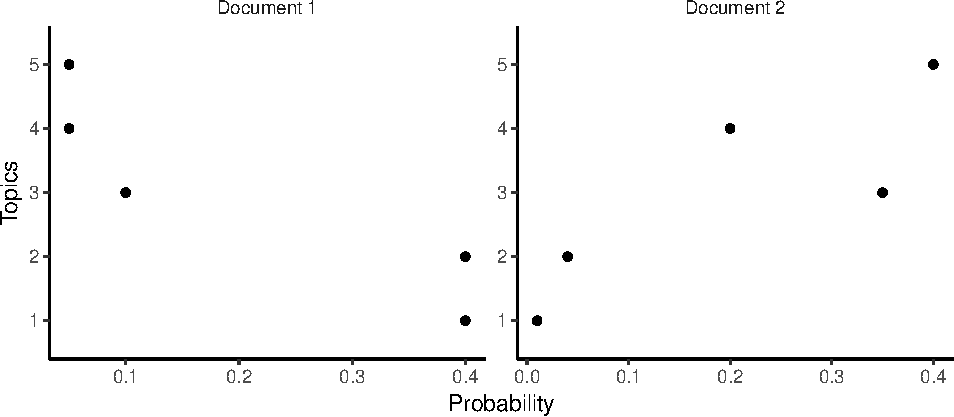
\includegraphics{svm-rmarkdown-article-example_files/figure-latex/topicsoverdocuments-1.pdf}
\caption{\label{fig:topicsoverdocuments}Probability distributions over
topics for two documents}
\end{figure}

Similarly, each topic could be considered a probability distribution
over terms. To choose the terms used in each document the speaker picks
terms from each topic in the appropriate proportion. For instance, if
there were ten terms, then one topic could be defined by giving more
weight to terms related to immigration; and some other topic may give
more weight to terms related to the economy (Figure
\ref{fig:topicsoverterms}).

\begin{figure}
\centering
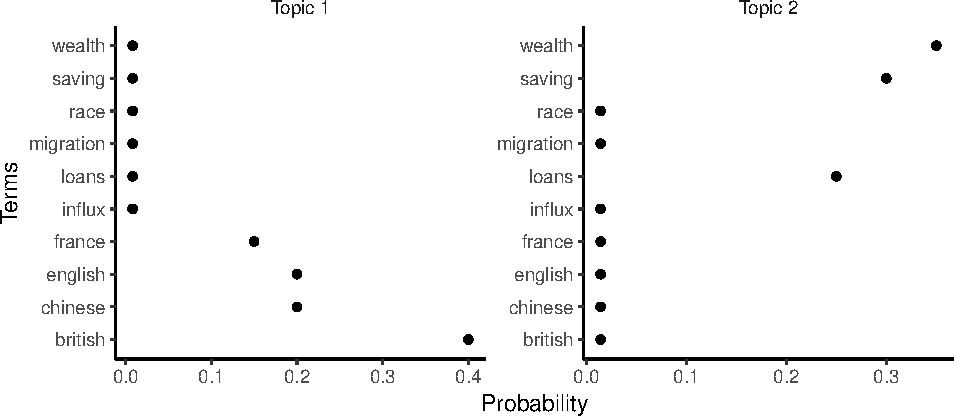
\includegraphics{svm-rmarkdown-article-example_files/figure-latex/topicsoverterms-1.pdf}
\caption{\label{fig:topicsoverterms}Probability distributions over terms}
\end{figure}

Following \citet{BleiLafferty2009}, \citet{blei2012} and
\citet{GriffithsSteyvers2004}, the process by which a document is
generated is more formally considered to be:

\begin{enumerate}
\def\labelenumi{\arabic{enumi}.}
\tightlist
\item
  There are \(1, 2, \dots, k, \dots, K\) topics and the vocabulary
  consists of \(1, 2, \dots, V\) terms. For each topic, decide the terms
  that the topic uses by randomly drawing distributions over the terms.
  The distribution over the terms for the \(k\)th topic is \(\beta_k\).
  Typically a topic would be a small number of terms and so the
  Dirichlet distribution with hyperparameter \(0<\eta<1\) is used:
  \(\beta_k \sim \mbox{Dirichlet}(\eta)\).\footnote{The Dirichlet
    distribution is a variation of the beta distribution that is
    commonly used as a prior for categorical and multinomial variables.
    If there are just two categories, then the Dirichlet and the beta
    distributions are the same. In the special case of a symmetric
    Dirichlet distribution, \(\eta=1\), it is equivalent to a uniform
    distribution. If \(\eta<1\), then the distribution is sparse and
    concentrated on a smaller number of the values, and this number
    decreases as \(\eta\) decreases. A hyperparameter is a parameter of
    a prior distribution.} Strictly, \(\eta\) is actually a vector of
  hyperparameters, one for each \(K\), but in practice they all tend to
  be the same value.
\item
  Decide the topics that each document will cover by randomly drawing
  distributions over the \(K\) topics for each of the
  \(1, 2, \dots, d, \dots, D\) documents. The topic distributions for
  the \(d\)th document are \(\theta_d\), and \(\theta_{d,k}\) is the
  topic distribution for topic \(k\) in document \(d\). Again, the
  Dirichlet distribution with the hyperparameter \(0<\alpha<1\) is used
  here because usually a document would only cover a handful of topics:
  \(\theta_d \sim \mbox{Dirichlet}(\alpha)\). Again, strictly \(\alpha\)
  is vector of length \(K\) of hyperparameters, but in practice each is
  usually the same value.
\item
  If there are \(1, 2, \dots, n, \dots, N\) terms in the \(d\)th
  document, then to choose the \(n\)th term, \(w_{d, n}\):

  \begin{enumerate}
  \def\labelenumii{\alph{enumii}.}
  \tightlist
  \item
    Randomly choose a topic for that term \(n\), in that document \(d\),
    \(z_{d,n}\), from the multinomial distribution over topics in that
    document, \(z_{d,n} \sim \mbox{Multinomial}(\theta_d)\).
  \item
    Randomly choose a term from the relevant multinomial distribution
    over the terms for that topic,
    \(w_{d,n} \sim \mbox{Multinomial}(\beta_{z_{d,n}})\).
  \end{enumerate}
\end{enumerate}

Given this set-up, the joint distribution for the variables is
(\citet{blei2012}, p.6):
\[p(\beta_{1:K}, \theta_{1:D}, z_{1:D, 1:N}, w_{1:D, 1:N}) = \prod^{K}_{i=1}p(\beta_i) \prod^{D}_{d=1}p(\theta_d) \left(\prod^N_{n=1}p(z_{d,n}|\theta_d)p\left(w_{d,n}|\beta_{1:K},z_{d,n}\right) \right).\]

Based on this document generation process the analysis problem,
discussed next, is to compute a posterior over \(\beta_{1:K}\) and
\(\theta_{1:D}\), given \(w_{1:D, 1:N}\). This is intractable directly,
but can be approximated (\citet{GriffithsSteyvers2004} and
\citet{blei2012}).

After the documents are created, they are all that we have to analyse.
The term usage in each document, \(w_{1:D, 1:N}\), is observed, but the
topics are hidden, or `latent'. We do not know the topics of each
document, nor how terms defined the topics. That is, we do not know the
probability distributions of Figures \ref{fig:topicsoverdocuments} or
\ref{fig:topicsoverterms}. In a sense we are trying to reverse the
document generation process -- we have the terms and we would like to
discover the topics.

If the earlier process around how the documents were generated is
assumed and we observe the terms in each document, then we can obtain
estimates of the topics (\citet{SteyversGriffiths2006}). The outcomes of
the LDA process are probability distributions and these define the
topics. Each term will be given a probability of being a member of a
particular topic, and each document will be given a probability of being
about a particular topic. That is, we are trying to calculate the
posterior distribution of the topics given the terms observed in each
document (\citet{blei2012}, p.~7):
\[p(\beta_{1:K}, \theta_{1:D}, z_{1:D, 1:N} | w_{1:D, 1:N}) = \frac{p\left(\beta_{1:K}, \theta_{1:D}, z_{1:D, 1:N}, w_{1:D, 1:N}\right)}{p(w_{1:D, 1:N})}.\]

The initial practical step when implementing LDA given a collection of
documents is to remove `stop words'. These are words that are common,
but that don't typically help to define topics. There is a common list
of stop words such as: ``a''; ``an''; and ``and''. However the exact
list used depends on research of focus. In the case of Australian
Hansard, these are words such as: ``australia''; ``australian''; and
``bill''. Punctuation and capitalisation is also typically removed. The
documents then need to then be transformed into a document-term-matrix.
This is essentially a table with a column of the number of times each
term appears in each document.

After the dataset is ready, the R \texttt{topicmodels} package of
\citet{Grun2011} can be used to implement LDA and approximate the
posterior. It can do this using Gibbs sampling or the variational
expectation-maximization algorithm. Following
\citet{SteyversGriffiths2006} and \citet{Darling2011}, the Gibbs
sampling process attempts to find a topic for a particular term in a
particular document, given the topics of all other terms for all other
documents. Broadly, it does this by first assigning every term in every
document to a random topic, specified by Dirichlet priors with
\(\alpha = \frac{50}{K}\) and \(\eta = 0.1\)
(\citet{SteyversGriffiths2006} recommends \(\eta = 0.01\)), where
\(\alpha\) refers to the distribution over topics and \(\eta\) refers to
the distribution over terms (\citet{Grun2011}, p.~7). It then selects a
particular term in a particular document and assigns it to a new topic
based on the conditional distribution where the topics for all other
terms in all documents are taken as given (\citet{Grun2011}, p.~6):
\[p(z_{d, n}=k | w_{1:D, 1:N}, z'_{d, n}) \propto \frac{\lambda'_{n\rightarrow k}+\eta}{\lambda'_{.\rightarrow k}+V\eta} \frac{\lambda'^{(d)}_{n\rightarrow k}+\alpha}{\lambda'^{(d)}_{-i}+K\alpha} \]
where \(z'_{d, n}\) refers to all other topic assignments;
\(\lambda'_{n\rightarrow k}\) is a count of how many other times that
term has been assigned to topic \(k\); \(\lambda'_{.\rightarrow k}\) is
a count of how many other times that any term has been assigned to topic
\(k\); \(\lambda'^{(d)}_{n\rightarrow k}\) is a count of how many other
times that term has been assigned to topic \(k\) in that particular
document; and \(\lambda'^{(d)}_{-i}\) is a count of how many other times
that term has been assigned in that document. Once \(z_{d,n}\) has been
estimated, then estimates for the distribution of words into topics and
topics into documents can be backed out.

This conditional distribution assigns topics depending on how often a
term has been assigned to that topic previously, and how common the
topic is in that document (\citet{SteyversGriffiths2006}). The initial
random allocation of topics means that the results of early passes
through the corpus of document are poor, but given enough time the
algorithm converges to an appropriate estimate.

The choice of the number of topics, \emph{k}, affects the results, and
must be specified \emph{a priori}. If there is a strong reason for a
particular number, then this can be used. Otherwise, one way to choose
an appropriate number is to use a test and training set process.
Essentially, this means running the process on a variety of possible
values for \emph{k} and then picking an appropriate value that performs
well.

One weakness of the LDA method is that it considers a `bag of words'
where the order of those words does not matter (\citet{blei2012}). It is
possible to extend the model to reduce the impact of the bag-of-words
assumption and add conditionality to word order. Additionally,
alternatives to the Dirichlet distribution can be used to extend the
model to allow for correlation. For instance, in Hansard topics related
the army may be expected to be more commonly found with topics related
to the navy, but less commonly with topics related to banking. This
motivates the use of the Structural Topic Model, described in the next
section.

\subsection{Structural Topic Model}\label{structural-topic-model}

The distinguishing aspect of the Structural Topic Model (STM) of
\citet{RobertsStewartAiroldi2016} is that it includes additional
information about documents. For instance, in general we usually have
some information about the author and date of a document. In the case of
Hansard, we know who was speaking and the date. STM allows this
additional information to affect the construction of topics, though
influencing either topical prevalence or topical content. That said, the
assumption that there is some document generation process is the same as
the LDA method, it is just that this process now includes metadata.

The STM is set-up to most easily include metadata to do with prevalence
and content. Prevalence relates to the topic proportions in each
document. For instance, we expect that topics related to the reasons for
Federation such as tariffs and trade should be more prevalent in those
earlier years than later. Similarly, we may expect topics to do with
terrorism to be more prevalent in recent years than in earlier ones.
Content relates to the words that make up each topic. For instance,
there are changes in the use of language over the period for which we
have data, and it would be better for these to not be responsible for
defining different topics rather than being part of the same topic.

The document generation process of \citet{Blei2003latent} discussed
earlier is modified slightly by \citet{RobertsStewartAiroldi2016}:

\begin{enumerate}
\def\labelenumi{\arabic{enumi}.}
\tightlist
\item
  The proportion of a document dedicated to a topic is drawn ``from a
  logistic-normal generalised linear model based on a vector of document
  covariates \(X_d\)'':
  \[\theta_d|X_d\gamma\sigma \sim logisticnormal(\mu = X_d\gamma, \sigma)\]
  ``where \(X_d\) is a 1-by-p vector, \(\gamma\) is a p-by-K - 1 matrix
  of coefficients and \(\sigma\) is K-1 by K-1 covariance matrix.''
  \textbf{THIS IS ALL QUOTES. NEED TO REWRITE.}
\item
  Given a document-level content covariate
\end{enumerate}

HERE

Following \citet{BleiLafferty2009}, \citet{blei2012} and
\citet{GriffithsSteyvers2004}, the process by which a document is
generated is more formally considered to be:

\begin{enumerate}
\def\labelenumi{\arabic{enumi}.}
\tightlist
\item
  There are For each topic, decide the terms that the topic uses by
  randomly drawing distributions over the terms. The distribution over
  the terms for the \(k\)th topic is \(\beta_k\). Typically a topic
  would be a small number of terms and so the Dirichlet distribution
  with hyperparameter \(0<\eta<1\) is used:
  \(\beta_k \sim \mbox{Dirichlet}(\eta)\).\footnote{The Dirichlet
    distribution is a variation of the beta distribution that is
    commonly used as a prior for categorical and multinomial variables.
    If there are just two categories, then the Dirichlet and the beta
    distributions are the same. In the special case of a symmetric
    Dirichlet distribution, \(\eta=1\), it is equivalent to a uniform
    distribution. If \(\eta<1\), then the distribution is sparse and
    concentrated on a smaller number of the values, and this number
    decreases as \(\eta\) decreases. A hyperparameter is a parameter of
    a prior distribution.} Strictly, \(\eta\) is actually a vector of
  hyperparameters, one for each \(K\), but in practice they all tend to
  be the same value.
\end{enumerate}

STM can be implented using the stm R package of
\citet{RobertsStewartAiroldiRPackage}.

Note that each of the states and the Commonwealth are treated
independently here. Future work could expand the model to better
understand, and allow, for correlation between them.

\subsubsection{Considering events}\label{considering-events}

{[}TBD{]}

\section{Results}\label{results}

\subsection{Political events}\label{political-events}

\begin{quote}
\emph{When you change the government, you change the country.} Paul
Keating.
\end{quote}

Change of government.

\subsection{Polling events}\label{polling-events}

\begin{quote}
\emph{The only poll that matters is the one on election day.} John
Howard.
\end{quote}

{[}TBD{]}

\subsection{Economic events}\label{economic-events}

Major economic changes.

{[}TBD{]}

\subsection{External events}\label{external-events}

\begin{quote}
\emph{Events, dear boy, events.} Attributed to Harold Macmillan.
\end{quote}

Major event such as 9/11 attacks, or economic change.

\section{Summary and conclusions}\label{summary-and-conclusions}

In this paper we examined

What could happen if we had longer terms. Eg GST needed multiple
generations of politicians but carbon tax couldn't because it was one
generation.

Text analysis has well-known biases and weaknesses and is a complement
to more detailed analysis such as qualitative methods and case studies.
We consider the results presented in this paper, as well as many of
those results of the larger text-as-data research program, as fitting
within findings based on other methods.

Future work - examine how it chagned during Federation

\newpage

\section{Appendix}\label{appendix}

\subsection{Document sources}\label{document-sources}

Where from?

Which years are being used (not non-OCRd)

\subsection{Dataset issues}\label{dataset-issues}

Which PDFs are missing or have no content, etc.

\begin{longtable}[]{@{}lllllll@{}}
\toprule
\begin{minipage}[b]{0.02\columnwidth}\raggedright\strut
year\strut
\end{minipage} & \begin{minipage}[b]{0.09\columnwidth}\raggedright\strut
I have this number in Reps\strut
\end{minipage} & \begin{minipage}[b]{0.10\columnwidth}\raggedright\strut
They say this number in Senate\strut
\end{minipage} & \begin{minipage}[b]{0.10\columnwidth}\raggedright\strut
They say this number in Reps\strut
\end{minipage} & \begin{minipage}[b]{0.07\columnwidth}\raggedright\strut
Difference in Reps\strut
\end{minipage} & \begin{minipage}[b]{0.11\columnwidth}\raggedright\strut
Comment\strut
\end{minipage} & \begin{minipage}[b]{0.31\columnwidth}\raggedright\strut
Source\strut
\end{minipage}\tabularnewline
\midrule
\endhead
\begin{minipage}[t]{0.02\columnwidth}\raggedright\strut
1902\strut
\end{minipage} & \begin{minipage}[t]{0.09\columnwidth}\raggedright\strut
106\strut
\end{minipage} & \begin{minipage}[t]{0.10\columnwidth}\raggedright\strut
93\strut
\end{minipage} & \begin{minipage}[t]{0.10\columnwidth}\raggedright\strut
107\strut
\end{minipage} & \begin{minipage}[t]{0.07\columnwidth}\raggedright\strut
1\strut
\end{minipage} & \begin{minipage}[t]{0.11\columnwidth}\raggedright\strut
Positive means I am missing some\strut
\end{minipage} & \begin{minipage}[t]{0.31\columnwidth}\raggedright\strut
\url{https://www.aph.gov.au/Parliamentary_Business/Statistics/Senate_StatsNet/General/sittingdaysyear}\strut
\end{minipage}\tabularnewline
\begin{minipage}[t]{0.02\columnwidth}\raggedright\strut
1908\strut
\end{minipage} & \begin{minipage}[t]{0.09\columnwidth}\raggedright\strut
93\strut
\end{minipage} & \begin{minipage}[t]{0.10\columnwidth}\raggedright\strut
84\strut
\end{minipage} & \begin{minipage}[t]{0.10\columnwidth}\raggedright\strut
91\strut
\end{minipage} & \begin{minipage}[t]{0.07\columnwidth}\raggedright\strut
-2\strut
\end{minipage} & \begin{minipage}[t]{0.11\columnwidth}\raggedright\strut
Negative means I have too many\strut
\end{minipage} & \begin{minipage}[t]{0.31\columnwidth}\raggedright\strut
\strut
\end{minipage}\tabularnewline
\begin{minipage}[t]{0.02\columnwidth}\raggedright\strut
1909\strut
\end{minipage} & \begin{minipage}[t]{0.09\columnwidth}\raggedright\strut
97\strut
\end{minipage} & \begin{minipage}[t]{0.10\columnwidth}\raggedright\strut
71\strut
\end{minipage} & \begin{minipage}[t]{0.10\columnwidth}\raggedright\strut
98\strut
\end{minipage} & \begin{minipage}[t]{0.07\columnwidth}\raggedright\strut
1\strut
\end{minipage} & \begin{minipage}[t]{0.11\columnwidth}\raggedright\strut
\strut
\end{minipage} & \begin{minipage}[t]{0.31\columnwidth}\raggedright\strut
\strut
\end{minipage}\tabularnewline
\begin{minipage}[t]{0.02\columnwidth}\raggedright\strut
1918\strut
\end{minipage} & \begin{minipage}[t]{0.09\columnwidth}\raggedright\strut
87\strut
\end{minipage} & \begin{minipage}[t]{0.10\columnwidth}\raggedright\strut
68\strut
\end{minipage} & \begin{minipage}[t]{0.10\columnwidth}\raggedright\strut
86\strut
\end{minipage} & \begin{minipage}[t]{0.07\columnwidth}\raggedright\strut
-1\strut
\end{minipage} & \begin{minipage}[t]{0.11\columnwidth}\raggedright\strut
\strut
\end{minipage} & \begin{minipage}[t]{0.31\columnwidth}\raggedright\strut
\strut
\end{minipage}\tabularnewline
\begin{minipage}[t]{0.02\columnwidth}\raggedright\strut
1920\strut
\end{minipage} & \begin{minipage}[t]{0.09\columnwidth}\raggedright\strut
113\strut
\end{minipage} & \begin{minipage}[t]{0.10\columnwidth}\raggedright\strut
76\strut
\end{minipage} & \begin{minipage}[t]{0.10\columnwidth}\raggedright\strut
114\strut
\end{minipage} & \begin{minipage}[t]{0.07\columnwidth}\raggedright\strut
1\strut
\end{minipage} & \begin{minipage}[t]{0.11\columnwidth}\raggedright\strut
\strut
\end{minipage} & \begin{minipage}[t]{0.31\columnwidth}\raggedright\strut
\strut
\end{minipage}\tabularnewline
\begin{minipage}[t]{0.02\columnwidth}\raggedright\strut
1921\strut
\end{minipage} & \begin{minipage}[t]{0.09\columnwidth}\raggedright\strut
92\strut
\end{minipage} & \begin{minipage}[t]{0.10\columnwidth}\raggedright\strut
79\strut
\end{minipage} & \begin{minipage}[t]{0.10\columnwidth}\raggedright\strut
93\strut
\end{minipage} & \begin{minipage}[t]{0.07\columnwidth}\raggedright\strut
1\strut
\end{minipage} & \begin{minipage}[t]{0.11\columnwidth}\raggedright\strut
\strut
\end{minipage} & \begin{minipage}[t]{0.31\columnwidth}\raggedright\strut
\strut
\end{minipage}\tabularnewline
\begin{minipage}[t]{0.02\columnwidth}\raggedright\strut
1934\strut
\end{minipage} & \begin{minipage}[t]{0.09\columnwidth}\raggedright\strut
36\strut
\end{minipage} & \begin{minipage}[t]{0.10\columnwidth}\raggedright\strut
22\strut
\end{minipage} & \begin{minipage}[t]{0.10\columnwidth}\raggedright\strut
35\strut
\end{minipage} & \begin{minipage}[t]{0.07\columnwidth}\raggedright\strut
-1\strut
\end{minipage} & \begin{minipage}[t]{0.11\columnwidth}\raggedright\strut
\strut
\end{minipage} & \begin{minipage}[t]{0.31\columnwidth}\raggedright\strut
\strut
\end{minipage}\tabularnewline
\begin{minipage}[t]{0.02\columnwidth}\raggedright\strut
1935\strut
\end{minipage} & \begin{minipage}[t]{0.09\columnwidth}\raggedright\strut
54\strut
\end{minipage} & \begin{minipage}[t]{0.10\columnwidth}\raggedright\strut
37\strut
\end{minipage} & \begin{minipage}[t]{0.10\columnwidth}\raggedright\strut
55\strut
\end{minipage} & \begin{minipage}[t]{0.07\columnwidth}\raggedright\strut
1\strut
\end{minipage} & \begin{minipage}[t]{0.11\columnwidth}\raggedright\strut
\strut
\end{minipage} & \begin{minipage}[t]{0.31\columnwidth}\raggedright\strut
\strut
\end{minipage}\tabularnewline
\begin{minipage}[t]{0.02\columnwidth}\raggedright\strut
1942\strut
\end{minipage} & \begin{minipage}[t]{0.09\columnwidth}\raggedright\strut
44\strut
\end{minipage} & \begin{minipage}[t]{0.10\columnwidth}\raggedright\strut
36\strut
\end{minipage} & \begin{minipage}[t]{0.10\columnwidth}\raggedright\strut
45\strut
\end{minipage} & \begin{minipage}[t]{0.07\columnwidth}\raggedright\strut
1\strut
\end{minipage} & \begin{minipage}[t]{0.11\columnwidth}\raggedright\strut
\strut
\end{minipage} & \begin{minipage}[t]{0.31\columnwidth}\raggedright\strut
\strut
\end{minipage}\tabularnewline
\begin{minipage}[t]{0.02\columnwidth}\raggedright\strut
1948\strut
\end{minipage} & \begin{minipage}[t]{0.09\columnwidth}\raggedright\strut
89\strut
\end{minipage} & \begin{minipage}[t]{0.10\columnwidth}\raggedright\strut
39\strut
\end{minipage} & \begin{minipage}[t]{0.10\columnwidth}\raggedright\strut
90\strut
\end{minipage} & \begin{minipage}[t]{0.07\columnwidth}\raggedright\strut
1\strut
\end{minipage} & \begin{minipage}[t]{0.11\columnwidth}\raggedright\strut
\strut
\end{minipage} & \begin{minipage}[t]{0.31\columnwidth}\raggedright\strut
\strut
\end{minipage}\tabularnewline
\begin{minipage}[t]{0.02\columnwidth}\raggedright\strut
1951\strut
\end{minipage} & \begin{minipage}[t]{0.09\columnwidth}\raggedright\strut
55\strut
\end{minipage} & \begin{minipage}[t]{0.10\columnwidth}\raggedright\strut
40\strut
\end{minipage} & \begin{minipage}[t]{0.10\columnwidth}\raggedright\strut
56\strut
\end{minipage} & \begin{minipage}[t]{0.07\columnwidth}\raggedright\strut
1\strut
\end{minipage} & \begin{minipage}[t]{0.11\columnwidth}\raggedright\strut
\strut
\end{minipage} & \begin{minipage}[t]{0.31\columnwidth}\raggedright\strut
\strut
\end{minipage}\tabularnewline
\begin{minipage}[t]{0.02\columnwidth}\raggedright\strut
1955\strut
\end{minipage} & \begin{minipage}[t]{0.09\columnwidth}\raggedright\strut
53\strut
\end{minipage} & \begin{minipage}[t]{0.10\columnwidth}\raggedright\strut
36\strut
\end{minipage} & \begin{minipage}[t]{0.10\columnwidth}\raggedright\strut
52\strut
\end{minipage} & \begin{minipage}[t]{0.07\columnwidth}\raggedright\strut
-1\strut
\end{minipage} & \begin{minipage}[t]{0.11\columnwidth}\raggedright\strut
\strut
\end{minipage} & \begin{minipage}[t]{0.31\columnwidth}\raggedright\strut
\strut
\end{minipage}\tabularnewline
\begin{minipage}[t]{0.02\columnwidth}\raggedright\strut
1974\strut
\end{minipage} & \begin{minipage}[t]{0.09\columnwidth}\raggedright\strut
64\strut
\end{minipage} & \begin{minipage}[t]{0.10\columnwidth}\raggedright\strut
64\strut
\end{minipage} & \begin{minipage}[t]{0.10\columnwidth}\raggedright\strut
62\strut
\end{minipage} & \begin{minipage}[t]{0.07\columnwidth}\raggedright\strut
-2\strut
\end{minipage} & \begin{minipage}[t]{0.11\columnwidth}\raggedright\strut
\strut
\end{minipage} & \begin{minipage}[t]{0.31\columnwidth}\raggedright\strut
\strut
\end{minipage}\tabularnewline
\begin{minipage}[t]{0.02\columnwidth}\raggedright\strut
1985\strut
\end{minipage} & \begin{minipage}[t]{0.09\columnwidth}\raggedright\strut
65\strut
\end{minipage} & \begin{minipage}[t]{0.10\columnwidth}\raggedright\strut
74\strut
\end{minipage} & \begin{minipage}[t]{0.10\columnwidth}\raggedright\strut
66\strut
\end{minipage} & \begin{minipage}[t]{0.07\columnwidth}\raggedright\strut
1\strut
\end{minipage} & \begin{minipage}[t]{0.11\columnwidth}\raggedright\strut
\strut
\end{minipage} & \begin{minipage}[t]{0.31\columnwidth}\raggedright\strut
\strut
\end{minipage}\tabularnewline
\begin{minipage}[t]{0.02\columnwidth}\raggedright\strut
1991\strut
\end{minipage} & \begin{minipage}[t]{0.09\columnwidth}\raggedright\strut
66\strut
\end{minipage} & \begin{minipage}[t]{0.10\columnwidth}\raggedright\strut
83\strut
\end{minipage} & \begin{minipage}[t]{0.10\columnwidth}\raggedright\strut
67\strut
\end{minipage} & \begin{minipage}[t]{0.07\columnwidth}\raggedright\strut
1\strut
\end{minipage} & \begin{minipage}[t]{0.11\columnwidth}\raggedright\strut
\strut
\end{minipage} & \begin{minipage}[t]{0.31\columnwidth}\raggedright\strut
\strut
\end{minipage}\tabularnewline
\begin{minipage}[t]{0.02\columnwidth}\raggedright\strut
1992\strut
\end{minipage} & \begin{minipage}[t]{0.09\columnwidth}\raggedright\strut
60\strut
\end{minipage} & \begin{minipage}[t]{0.10\columnwidth}\raggedright\strut
76\strut
\end{minipage} & \begin{minipage}[t]{0.10\columnwidth}\raggedright\strut
44\strut
\end{minipage} & \begin{minipage}[t]{0.07\columnwidth}\raggedright\strut
-16\strut
\end{minipage} & \begin{minipage}[t]{0.11\columnwidth}\raggedright\strut
\strut
\end{minipage} & \begin{minipage}[t]{0.31\columnwidth}\raggedright\strut
\strut
\end{minipage}\tabularnewline
\begin{minipage}[t]{0.02\columnwidth}\raggedright\strut
1993\strut
\end{minipage} & \begin{minipage}[t]{0.09\columnwidth}\raggedright\strut
47\strut
\end{minipage} & \begin{minipage}[t]{0.10\columnwidth}\raggedright\strut
53\strut
\end{minipage} & \begin{minipage}[t]{0.10\columnwidth}\raggedright\strut
46\strut
\end{minipage} & \begin{minipage}[t]{0.07\columnwidth}\raggedright\strut
-1\strut
\end{minipage} & \begin{minipage}[t]{0.11\columnwidth}\raggedright\strut
\strut
\end{minipage} & \begin{minipage}[t]{0.31\columnwidth}\raggedright\strut
\strut
\end{minipage}\tabularnewline
\begin{minipage}[t]{0.02\columnwidth}\raggedright\strut
1994\strut
\end{minipage} & \begin{minipage}[t]{0.09\columnwidth}\raggedright\strut
69\strut
\end{minipage} & \begin{minipage}[t]{0.10\columnwidth}\raggedright\strut
80\strut
\end{minipage} & \begin{minipage}[t]{0.10\columnwidth}\raggedright\strut
68\strut
\end{minipage} & \begin{minipage}[t]{0.07\columnwidth}\raggedright\strut
-1\strut
\end{minipage} & \begin{minipage}[t]{0.11\columnwidth}\raggedright\strut
\strut
\end{minipage} & \begin{minipage}[t]{0.31\columnwidth}\raggedright\strut
\strut
\end{minipage}\tabularnewline
\begin{minipage}[t]{0.02\columnwidth}\raggedright\strut
1995\strut
\end{minipage} & \begin{minipage}[t]{0.09\columnwidth}\raggedright\strut
71\strut
\end{minipage} & \begin{minipage}[t]{0.10\columnwidth}\raggedright\strut
78\strut
\end{minipage} & \begin{minipage}[t]{0.10\columnwidth}\raggedright\strut
70\strut
\end{minipage} & \begin{minipage}[t]{0.07\columnwidth}\raggedright\strut
-1\strut
\end{minipage} & \begin{minipage}[t]{0.11\columnwidth}\raggedright\strut
\strut
\end{minipage} & \begin{minipage}[t]{0.31\columnwidth}\raggedright\strut
\strut
\end{minipage}\tabularnewline
\begin{minipage}[t]{0.02\columnwidth}\raggedright\strut
1997\strut
\end{minipage} & \begin{minipage}[t]{0.09\columnwidth}\raggedright\strut
79\strut
\end{minipage} & \begin{minipage}[t]{0.10\columnwidth}\raggedright\strut
82\strut
\end{minipage} & \begin{minipage}[t]{0.10\columnwidth}\raggedright\strut
76\strut
\end{minipage} & \begin{minipage}[t]{0.07\columnwidth}\raggedright\strut
-3\strut
\end{minipage} & \begin{minipage}[t]{0.11\columnwidth}\raggedright\strut
\strut
\end{minipage} & \begin{minipage}[t]{0.31\columnwidth}\raggedright\strut
\strut
\end{minipage}\tabularnewline
\begin{minipage}[t]{0.02\columnwidth}\raggedright\strut
1998\strut
\end{minipage} & \begin{minipage}[t]{0.09\columnwidth}\raggedright\strut
56\strut
\end{minipage} & \begin{minipage}[t]{0.10\columnwidth}\raggedright\strut
57\strut
\end{minipage} & \begin{minipage}[t]{0.10\columnwidth}\raggedright\strut
54\strut
\end{minipage} & \begin{minipage}[t]{0.07\columnwidth}\raggedright\strut
-2\strut
\end{minipage} & \begin{minipage}[t]{0.11\columnwidth}\raggedright\strut
\strut
\end{minipage} & \begin{minipage}[t]{0.31\columnwidth}\raggedright\strut
\strut
\end{minipage}\tabularnewline
\begin{minipage}[t]{0.02\columnwidth}\raggedright\strut
2000\strut
\end{minipage} & \begin{minipage}[t]{0.09\columnwidth}\raggedright\strut
71\strut
\end{minipage} & \begin{minipage}[t]{0.10\columnwidth}\raggedright\strut
71\strut
\end{minipage} & \begin{minipage}[t]{0.10\columnwidth}\raggedright\strut
73\strut
\end{minipage} & \begin{minipage}[t]{0.07\columnwidth}\raggedright\strut
2\strut
\end{minipage} & \begin{minipage}[t]{0.11\columnwidth}\raggedright\strut
\strut
\end{minipage} & \begin{minipage}[t]{0.31\columnwidth}\raggedright\strut
\strut
\end{minipage}\tabularnewline
\begin{minipage}[t]{0.02\columnwidth}\raggedright\strut
2002\strut
\end{minipage} & \begin{minipage}[t]{0.09\columnwidth}\raggedright\strut
68\strut
\end{minipage} & \begin{minipage}[t]{0.10\columnwidth}\raggedright\strut
60\strut
\end{minipage} & \begin{minipage}[t]{0.10\columnwidth}\raggedright\strut
69\strut
\end{minipage} & \begin{minipage}[t]{0.07\columnwidth}\raggedright\strut
1\strut
\end{minipage} & \begin{minipage}[t]{0.11\columnwidth}\raggedright\strut
\strut
\end{minipage} & \begin{minipage}[t]{0.31\columnwidth}\raggedright\strut
\strut
\end{minipage}\tabularnewline
\begin{minipage}[t]{0.02\columnwidth}\raggedright\strut
2003\strut
\end{minipage} & \begin{minipage}[t]{0.09\columnwidth}\raggedright\strut
74\strut
\end{minipage} & \begin{minipage}[t]{0.10\columnwidth}\raggedright\strut
64\strut
\end{minipage} & \begin{minipage}[t]{0.10\columnwidth}\raggedright\strut
75\strut
\end{minipage} & \begin{minipage}[t]{0.07\columnwidth}\raggedright\strut
1\strut
\end{minipage} & \begin{minipage}[t]{0.11\columnwidth}\raggedright\strut
\strut
\end{minipage} & \begin{minipage}[t]{0.31\columnwidth}\raggedright\strut
\strut
\end{minipage}\tabularnewline
\begin{minipage}[t]{0.02\columnwidth}\raggedright\strut
2004\strut
\end{minipage} & \begin{minipage}[t]{0.09\columnwidth}\raggedright\strut
58\strut
\end{minipage} & \begin{minipage}[t]{0.10\columnwidth}\raggedright\strut
49\strut
\end{minipage} & \begin{minipage}[t]{0.10\columnwidth}\raggedright\strut
59\strut
\end{minipage} & \begin{minipage}[t]{0.07\columnwidth}\raggedright\strut
1\strut
\end{minipage} & \begin{minipage}[t]{0.11\columnwidth}\raggedright\strut
\strut
\end{minipage} & \begin{minipage}[t]{0.31\columnwidth}\raggedright\strut
\strut
\end{minipage}\tabularnewline
\begin{minipage}[t]{0.02\columnwidth}\raggedright\strut
2012\strut
\end{minipage} & \begin{minipage}[t]{0.09\columnwidth}\raggedright\strut
63\strut
\end{minipage} & \begin{minipage}[t]{0.10\columnwidth}\raggedright\strut
57\strut
\end{minipage} & \begin{minipage}[t]{0.10\columnwidth}\raggedright\strut
67\strut
\end{minipage} & \begin{minipage}[t]{0.07\columnwidth}\raggedright\strut
4\strut
\end{minipage} & \begin{minipage}[t]{0.11\columnwidth}\raggedright\strut
\strut
\end{minipage} & \begin{minipage}[t]{0.31\columnwidth}\raggedright\strut
\strut
\end{minipage}\tabularnewline
\bottomrule
\end{longtable}

\subsection{Example workflow}\label{example-workflow}

Example of the workflow from PDF to text

\subsection{PDF to CSV issues}\label{pdf-to-csv-issues}

Insert graph of stop words over time.

\subsection{Selection of number of
topics}\label{selection-of-number-of-topics}

\subsection{Robustness of results}\label{robustness-of-results}

Here we change the number of sitting days considered either side of an
event. The results in the main section of the paper are for the nearest
ten days either side of an event. Here are show that the results are
essentially the same if the nearest one, two, five, and twenty days
either side of an event.

\newpage




\newpage
\singlespacing 
\renewcommand\refname{References}
\bibliography{../bibliography.bib}

\end{document}
